\chapter{METHODOLOGY}
In this chapter, the methodology is detailed as follows. 
First, we describe the architecture of the model. 
Second, we explain the \acrshort{mlm} pre-training loss functions used in this experiment.
Third, the details of \acrshort{pos} tagging are provided. 
Fourth, we outline the datasets used in this experiment. 
Fifth, we provide details on the visual question answering setup.
Lastly, we provide implementation detail for the pre-training model.

\begin{figure}[h]
    \caption{Overall methodology}
    \label{fig:overview}
    Pre-training the model with a \acrshort{mlm} task by masking tokens based on the \acrshort{pos} in the image captions.
    \begin{center}
        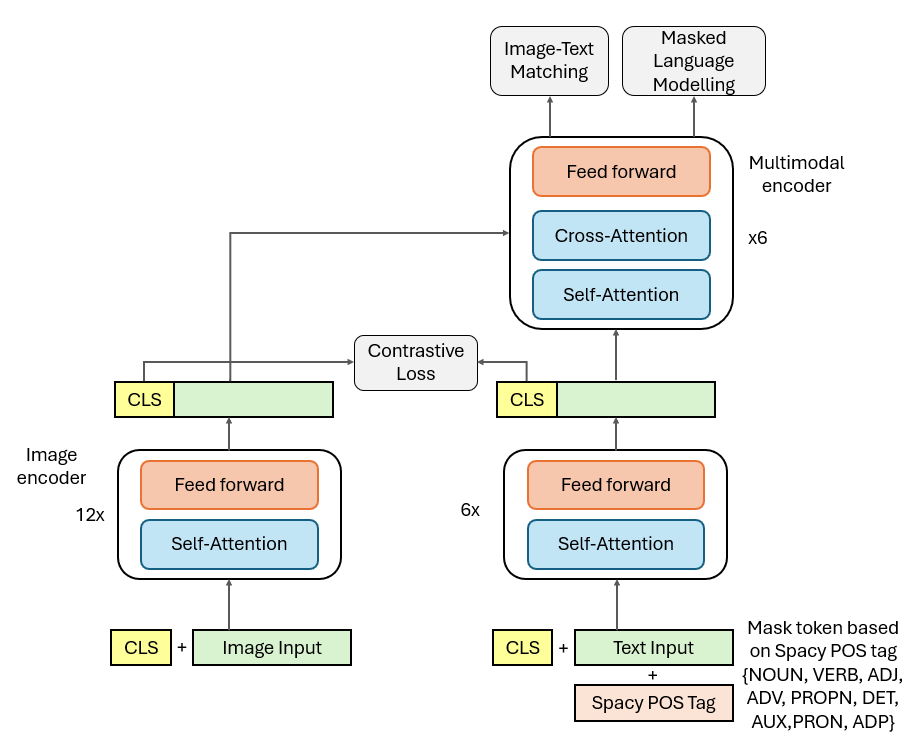
\includegraphics[width=0.8\textwidth]{Images/overview.png}
    \end{center}
    \small
\end{figure}

\section{Model architecture}
As shown in Figure \ref{fig:overview}, our model includes three main components: an image encoder, a text encoder, and a multimodal encoder. 
The first component is the image encoder, for which we use ViT \cite{vit}, modified following \cite{clip}, as the image encoder in this experiment. 
The second component is the text encoder, which employs a transformer architecture as BERT \cite{bert} to encode image captions.
The final component is the multimodal encoder, where \acrshort{vl} interactions occur.

Given a training dataset \(D\) consisting of image-text pairs \((I_i, T_i) \in D\), where \(I_i\) is the image and \(T_i\) is the image caption of the \(i\)-th image, each image is first encoded as a sequence of tokens \(\{v_{cls}, v_1, \dots, v_n\}\) using ViT \cite{vit}. 
Here, \(v_{cls}\) represents the embedding of the [CLS] token prepended to the image patch sequence. 
In this experiment, the image encoder was initialized with ViT-B-32 pre-trained on ImageNet-21K \cite{imagenet}.
Next, we use a 6-layer transformer, randomly initialized, to encode the image caption \(T_i\) into text embeddings \(\{w_{cls}, w_1, \dots, w_n\}\), where \(w_{cls}\) is the embedding of the [CLS] token. 
Finally, both text and image encodings are passed through the multimodal encoder to fuse both inputs, producing multimodal encodings. 
For the multimodal encoder, a cross-attention layer is used, where both keys and values are the image encodings, and the text encoding serves as the query in the cross-attention layer.


% Cross Attention using Image = K, V Text as a query.
% Thought: The image encoder choice can be change based on training speec.
\section{Pre-training objectives}
In this work, we pre-train our model with three objectives: \acrfull{mlm}, \acrfull{itc} and \acrfull{itm}.
\subsection{Mask language modelling}
Our model is trained with the \acrshort{mlm} task. 
Typically, a percentage of tokens \(\{w_1, \dots, w_T\}\) are replaced with a special [MASK] token to create a masked caption \(T^{\text{mask}}\). 
However, in this work, the masked tokens are selected based on \acrshort{pos} type instead of randomly masking. 
The model is then trained to predict the original tokens at the masked positions, conditioned on both the unmasked tokens in \(T^{\text{mask}}\) and the visual features of \(I\) as \(p^{\text{mask}}(I, T^{\text{mask}})\).
Let \(y^{\text{mask}}\) be a one-hot vector representing the ground-truth vocabulary for the masked token, where the masked token has a probability of 1. 
The model’s objective is to minimize the cross-entropy \(\mathbf{H}\), given by:
\[
    \mathcal{L}_{\text{MLM}} = \mathbf{H}(y^{\text{mask}}, p^{\text{mask}}(I, T^{\text{mask}})S))
\]

\subsection{Image-text contrative learning}
To improve each unimodal encoders representation, we use \acrshort{itc} to improve alignment of each modality.
\acrshort{itc} aims to improve alignment by maximize similarity score of image and text from the same pair with score function \(s(I, T) = v_{cls}^\top w_{cls}\), and minimize similarity score of image and text not from its pair.
We then calculate softmax-normalized similiarity score for each image to any text and each text to any image, identified as image-to-text \(p^{i2t} \in \mathbb{R}^{M}\) and text-to-image \(p^{t2i} \in \mathbb{R}^{M}\) score as:
\[
    p^{i2t}_i(I) = \frac{ \exp{(s(I,T_i))/\tau} }{ \sum_{m=1}^{M}\exp{(s(I,T_m)/\tau} }, \quad p^{t2i}_i(T) = \frac{ \exp{(s(T,I_i))/\tau} }{ \sum_{m=1}^{M}\exp{(s(T,I_m)/\tau} }
\]
where \(\tau\) is a learnable temperature parameter. Let \( y^{i2t}(I) \in \{0,1\}^M \) and \( y^{t2i}(T) \in \{0,1\}^M \) be a ground truth with probability of 1 at a position of same pair, and probability of 0 on the otherhand.
The \acrshort{itc} loss is calculated as cross-entropy \(\mathbf{H}\) between \(p\) and \(y\):
\[
    \mathcal{L}_{\text{ITC}} = \frac{1}{2}(\mathbf{H}(y^{i2t},p^{i2t}) + \mathbf{H}(y^{t2i},p^{t2i}))
\]
\subsection{Image-text matching}
\section{Part of speech tagging}


\section{Pre-training dataset}
We pre-trained the model on the Conceptual Captions dataset \cite{conceptual-caption}, which consists of 3.3 million image-text pairs. 
In Conceptual Captions dataset, an automated process was used to select, filter, and refine these image-caption pairs to ensure they are clear, informative, and suitable for effective model training.

\section{Evaluation}
In this work, we evaluate each model trained with different types of \acrshort{pos} masking using image-text retrieval and visual question answering tasks. 
The details of the evaluation methods and datasets are described in this section.


\subsection{Image-text retrieval}
For the image-text retrieval task, we evaluate the effect of masking on each \acrshort{pos} category by performing zero-shot evaluations on the Flickr30K \cite{flickr30k} and VALSE \cite{valse} datasets for both image-to-text and text-to-image retrieval. 
The Flickr30K dataset is used to assess the model's overall performance in retrieval tasks. 
For a deeper understanding, the VALSE dataset provides a breakdown of linguistic phenomena into six categories: existence, plurality, counting, relation, action, and coreference. 
Each image caption in the VALSE dataset also includes a "foil" version, in which words related to each caption category are altered. 
This approach enables us to analyze how different \acrshort{pos} masking strategies impact the model retrieval performance and the alignment between visual and textual representations.

\subsection{Visual question answering}
For visual question answering task, we assess each model with

% \section{Implementation Detail}
% BF16 datatype